\documentclass{article}
\usepackage{graphicx}
\usepackage{xcolor}
\usepackage[margin=3cm]{geometry} % margins might need to change in the future check with professor adam 
\setlength{\parindent}{0pt}
\usepackage{pgfgantt}

\usepackage{times}
\usepackage{fancyhdr,graphicx,amsmath,amssymb}
\usepackage[ruled,vlined]{algorithm2e}
\include{pythonlisting}


\begin{document}


\section{Literature Review: }

\subsection{ Introduction: }
  
Humanity has spent millennia observing the world, creating concepts that describe the variables, such as mass and force, to derive laws. In physics, like with
all human endeavours, new discoveries and ways of thought are based upon previous works, creating
a natural bias in the way new problems are approached. All existing theories, are therefore
somewhat biased, this combined with our pre-existing bias in our biological brains, can introduce some
hurdles to our future progress \cite{Wood2022} \cite{Schmidt2009}.\\

In the 17th Century, Kepler had gotten his hands on the word’s most precise data tables on the orbits
on planets, using this he spent close to half a decade, and after numerous unsuccessful
attempts, he had began a scientific revolution at the time, describing Mar’s orbit to be an ellipse \cite{kepler}.
In essence, scientists throughout history, much like Kepler, have spent a great deal of time, discovering
the right expressions to match the relevant data they have, this at it’s core is symbolic regression. Now,
a few centuries later, even with exponential increases in orders of magnitude in our capability to perform
calculations through computers, the process of discovering natural laws and the way to express them,
has to some extent resisted automation.\\


One of the core challenges of physics and artificial intelligence, is finding analytical relations automatically, discovering a symbolic expression that accurately matches the data from an unknown function.
This problem, due to it’s nature, is NP-hard \cite{Hope2023} in principle. The vastness of the space
of mathematical constants, adds to the difficulty. 
This literatire review aims to present the recent advances in discovery of emphirical laws through data powered by artificial intelligence. It focuses on methodoogies that dimish human bias through seeking solutions without assumptions. We will explore various techniques employed to achieve these goals, which includes reducing the search space, and analyse the effectivness of these methods.\\  

\begin{figure}[h] 
    \centering
    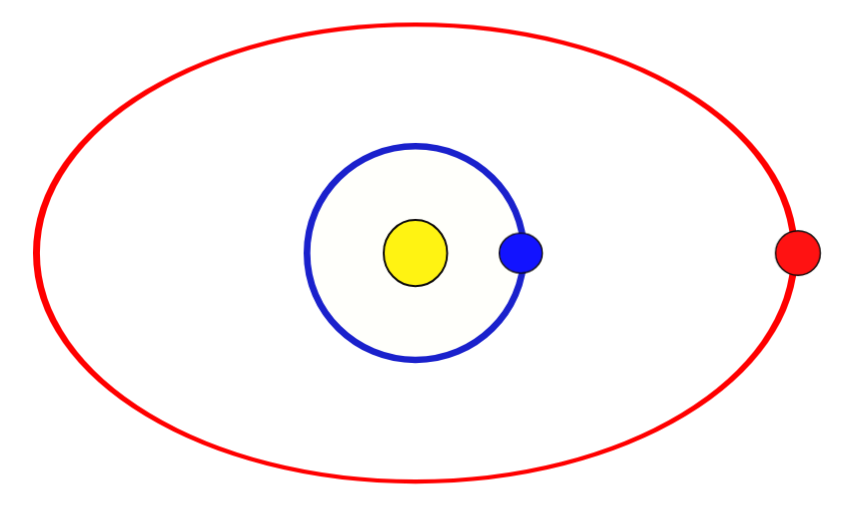
\includegraphics[width=7cm]{Sun_Mars_Orbit} 
    \caption{This is the orbit of Earth and Mars around the Sun.}
    \label{fig:Orbit} 
\end{figure}


\subsection{Symbolic Regression: }

Symbolic regression, is a technique that analyses and searches over the space of traceable mathematical
expressions to find the best fit for a data set. By not requiring prior information about the model,
it is unbiased. There are a plethora of various strategies that have been implemented in solving for
empirical laws \cite{Schmidt22009}, we will explore some of them below. It is also worth mentioning, that unlike other
well-known techniques for regression, (eg: neural networks), that are essentially black boxes, symbolic
regression, aims to extract white-box models and is easy to analyse.\\

\begin{center} 
  \textbf {\Large  Brute Force:}
\end{center}
Symbolic Regression (SR), is interpretable \cite{Aldeia2022}, unlike Neural Networks (NN), which are often considered more explainable. The difference is interpretability allows us to comprehend how the model works,
like observing how gears move in a glass box, while explainable means you get an overview of why a
certain output was achieved, even without knowing the full nuances of it’s inner workings.\\

There however, are some challenges associated with SR, in comparison to function fitting (NN). SR,
starts with nothing, a blank slate, and it has to learn the entire expression \cite{Cranmer2020}, unlike function fitting
which just tweaks an already existing function. The exponential search space \cite{Worm2014} , causes it to be
extremely computationally expensive to explore all possibilities. This combined with the face that,
most optimisation algorithms expect a smooth search space \cite{Makke2024}, however SR lack’s smooth interpolation, small changes in the potential solutions (expression), ie: $ x3 and x3 + 0.1$ can significantly alter
the the output. Finally, if the nature of the problem is badly posed \cite{Rivero2022}, there might potentially be
multiple solutions to the same data. Imagine trying to find a single polynomial equation with only two
points of data, the need to balance finding accurate expressions with finding the most simplistic and
generalisable fit, is sometimes troublesome.\\

The brute force approach of simply trying all possible combinations of symbolic expressions within some defined space. The model will subsequently increase the complexity over time, and will stop when either the fitting errors lowers below some defined limit or exceeds the upper limit of runtime. While in theory can solve all of our problems, in practise takes longer than the age of our universe to finish. In essence it's like searching for a singular drop in the ocean. Thankfully, there are some ways of pruning the search space, and drastically reducing the time taken to solve for the most accurate expression. \\ 

\begin{center} 
  \textbf {\Large Partial Derivatives:}
\end{center}

Partial derivatives, of some function f, with multiple variables such as x and y, is it's dervative with respect to one of those two variables, while the other variables in the function are kept constant. Formally, given a function with two or more variables, $f(x_1, x_2, \ldots, x_n) $, the partial derivative of $f$ with respect to $x_i$, where $x_i$ is some value $x$ in $(x_1, x_2, \ldots, x_i, \ldots, x_n)$, gives the rate of change of $f$ with respect to $x_i$. It is calculated by taking the ith derivative of $f$ with respect to $x_i$, whilst holding the other variables fixed. \cite{Stewart2012} \cite{Smith2012} \\

The partial derivative of a function $f(x,y)$ with respect to $x$ is denoted $\frac{\partial f}{\partial x}$ \cite{Kelly2021} and is defined: \\ 

\begin{center}

  $\frac{\partial f}{\partial x} = \lim_{h \to 0} \left[ \frac{f(x+h, y) - f(x,y)}{h} \right]$
\end{center}


Once you pass in the experimental data, you can pre-process the data, using calculated partial derivatives, for every pair of existing variables. Many physical laws, involve rates of change, and partial
derivatives help us represent them. Furthermore it also guides the search process, as the algorithm can
use the derivative to accurately represent the underlying laws involved. Through comparing how well
the partial derivatives derived through the experimental data compared to the potential expression,
the algorithm can assess the accuracy and feasibility of the expressions involved. This strategy can
even be extended to prune the search space further, this could be achieved through incorporating
knowledge of physics into the constraints for the partial derivatives. These concepts will be illustrated
with an example below.\\


Consider a iron rod, that has been heated up, such that it is hotter on one side than the other. Now it is intuitive to say that closer to the heat source, the temperature will be higher than further along the rod, where it will be colder. We can illustrate this temperature distribution with a function:  \\

\begin{center}
$T(x,y,z)$
\end{center}

where T is the temperature at a point in the rod, and (x,y,z) are the coordinates along the axis in 3 dimensions. This leads to these 3 partial derivatives: \\ 

\begin{center}
 $\frac{\partial T}{\partial x}, \  \frac{\partial T}{\partial y}, \  \frac{\partial T}{\partial z}$
\end{center}

These partial derivatives, gives us information about the direction and magnitude of heat flow at various points on the rod. The algorithm then searches for an equation T(x,y,z), that sufficiently predicts the observed temperature distribution and it's partial derivatives, deriving laws such as the heat transfer equations, or elasticity relationships.\\ 

\begin{center}
$\frac{\partial T}{\partial t} = \alpha \nabla^2 T$
\end{center}



Through using partial derivatives, we have in essence redefined the search criteria for the algorithm, through it's measure of the accuracy in comparison of potential solutions over the invariants represented in the experimental data \cite{Kelly2021} . This also leads to the pleasant finding, that it can additionally capture relationships that represent other identities of the system, beyond invariants and heat transfer equations. \\ 

You can subtly guide the type of laws that such an algorithm finds, by selectively picking the variables to input into the algorithm,. For example providing velocities and force to find laws of motion. \\ 





\begin{center} 
  \textbf {\Large Dimensional Analysis:}
\end{center}

Dimensional Analysis is a method of solving problems usually in maths and physics, where we analyse
the relationships between different physical quantities, by comparing their ”units.” It is a powerful
method of reducing the complexity of systems, enabling engineers and scientists to analyse problems
that we can’t even pose, much less solve the equations of \cite{Longo2021}.\\

Using the fact that numerous questions in science can be simplified by requiring the dimensions/units
of the right and left hand side of the expression to be equal, we can transform the question into
a smaller number of variables, which all have no dimension \cite{Blasiak2012}. It has been automated to find the integer powers of expressions and has proven to be useful especially when the power is an irrational number.\\

Here is a general strategy that showcases how dimensional analysis can be used:\\

Let's say we have a variable in an equation that can be broken down into it's fundamental units, such as (second, kilograms, ampere ...) to various powers. We can then take this, and represent each of the units as vectors, such that each of the fundamental units, is assigned a dimension, and it's important to note, this then allows us to represent any physical quantity as a product of these units, so let us construct a vector $v$, with $3$ integers, where each corresponding integer represents the power of each of the fundamental units.\\ 

Given that we want to derive an expression, such as $y = f(x_1, \dots, x_n)$  we can then create some matrix $M$. Each of the columns of the given matrix, is the unit vector $v$ of the corresponding variable $x_i$. We then need to define another vector to represent the units of y, which will be called $z$. If we let the solution be some vector $s$, solving $Ms = z$, this then lets us raise the powers on both sides, to elevate the independent variables, to make this equation dimensionally consistent.\\ 

Taking the null space of the matrix $M$, where $MV = 0$, allows us a basis to create a dimensionless group, allows for a simplification of the problem.\\

This is also more intuitive to understand physical phenomena, the nature of physics comprehension, making this vital in further understanding derived laws, making the process easier to explain and understand \cite{Taber2009}. Therefore, this is a crucial tool, for cultivating a deeper understanding of physics effectively \cite{Tenachi2023}. \\






\begin{center} 
  \textbf {\Large Genetic Programming:}
\end{center}


Genetic programming (GP), is a special evolutionary algorithmic technique, where the individuals are seen as programs that evolve, starting for a population, is iteratively "evolved," transforming the populations of individual programs, intro other populations. This new generation of programs are created using some genetic operations or survival criteria, mimicking natural evolutionary condition on earth.\\ 

A very basic overview, shows that genetic programming algorithms, consists of initializing the population, then evaluation of the said population through some predefined metrics and functions, followed by selection of the fittest programs based on the score given by the metric, and "genetic operation," such as reproduction, mutation and cross-over. The algorithm then iterates these steps thousands of times, through many generations, and finally terminates once the desired result has been achieved.\\

We can use genetic programming, and tweak the algorithm, and combine it with symbolic regression, to help us derive laws. \\

Consider modelling the various potential formulas as a tree, which is composed of various functions in the nodes. These functions can vary from arithmetic operations  , mathematical functions, or defined unique operators. Then we can program the fitness function \cite{Angeline1994}, and use it to measure how well the given potential expression in the population compares with the given databases, and given the nature of genetic programming, the better performing functions are more likely to be passed down into the next generation. Then after many iterations, we can give the solution with the best performance. \\ 

There are various ways to implement the fitness function, and for example we can use a criteria like this, along with mean squared error \cite{Liddle2009}:\\

\begin{center}
  $V = 2X + N \cdot ln(M/N) $
\end{center}

Here M is the mean squared error, and N is the number of data points, X is the number of parameters used on the genetic programming algorithm. The lower the value of V is, the better the model performs. The performance of this stratergy can then be evaluated with various other metrics, to judge how well the algorithm performs. \\ 











\subsection{ Conclusion: }

To efficiently traverse the search space, these are some of the various techniqies that could be utilised to reduce its dimensionality. An algorithm combining these stratergies offers a optimised approach to deriving emphirical laws while maintaining generality. This review explored diverse methods for designing and refining the search space. \\   




\section{Technical Progress: }

This section describes the relevent implementations that are completed as of 10 December 2024.\\ 

\subsection{Momentum Laws: }

To generate the dataset, I chose 100 data points, and created two variables mass (M) and acceleration (a), each represented in two dimensions. Then the data points were generated using $numpy.random.randn$ function. The force (F), was then calculated to be the produce of these two data sets. Mass and acceleration were concatenated along the same axis using $numpy.concatenate$, resulting in a combined dataset. This is partially because the model used here, $PySRRegressor$ expects a single array as input, and this helps highlight the relationship between these variables to the symbolic regression algorithm.\\ 

Then model performed symbolic regression, configured with 40 iterations along with a customer loss function, taken to be the squred diffrence between the prediction and the target variable. \\ 

\begin{center}
  
  $$
  {\boldsymbol{\mathcal{L}(\hat{x}, x) = (\hat{x} - x)^2}}
$$

\end{center}


The model was trained on this dataset, upon termination, it produced a list of potential candidate formulae, from which I manually identified the correct expression, $F = m \dot a$. \\



\begin{algorithm}[H]
\SetAlgoLined
\KwResult{A symbolic representation approximating \( F = M \cdot A \)}
\textbf{Initialization:} \\
Generate random data for mass (\( M \)) and acceleration (\( A \))\;
Compute target force values: \( F = M \cdot A \)\;
Combine \( M \) and \( A \) into input matrix \( X \)\;

\While{Symbolic regression process}{
  Train the symbolic regression model with the following settings:\;
  \textbf{Binary operators:} Multiplication (\(*\))\;
  \textbf{Unary operators:} None\;
  \textbf{Loss function:} Mean squared error between predictions and targets\;
  \textbf{Iterations:} 40\;

  \eIf{Current symbolic representation improves loss}{
   Update the symbolic model\;
   Save the current best expression\;
   }{
   Continue exploration of new symbolic expressions\;
  }
 }
\caption{Symbolic Regression for \( F = M \cdot A \)}
\end{algorithm}

\\
\\

Similarly, the other laws of momentum, were also dervied using this approach. \\ 
\\

\begin{align} \label{eq:impulse_momentum}
\mathbf{F} \Delta t &= \Delta \mathbf{p} = m(\mathbf{v}_f - \mathbf{v}_i) \\
m_1 \mathbf{v}_{1,i} + m_2 \mathbf{v}_{2,i} &= m_1 \mathbf{v}_{1,f} + m_2 \mathbf{v}_{2,f}
\end{align} 
%\subsection{Optimising the Symbolic Regression Algorithm: }

%\subsection{Neural Networks: }

%\subsection{ White Box models: }

\subsection{Pendulum Laws:}

The data is generated using numpy. The simulation involves, Euler's method to solve the pendulum's equation of motion. Through taking small and discrete steps, the method approximates the solution. The equation for a simple pendulum is given by: \\

\begin{center}
\begin{equation}
\alpha = -\frac{g}{L} \sin(\theta)
\end{equation}
\end{center}

\begin{description}
    \item[\(\alpha\)] angular acceleration (\(\text{rad/s}^2\))
    \item[\(g\)] acceleration due to gravity (\(\text{m/s}^2\))
    \item[\(L\)] length of the pendulum (\(\text{m}\))
    \item[\(\theta\)] angular displacement (\(\text{rad}\))
\end{description}

The Euler technique approximates the changes in angular velocity and displacement over some small step in time, as follows:\\

\begin{center}
\begin{align} 
\omega_{i+1} &= \omega_i + \alpha_i \Delta t \\
\theta_{i+1} &= \theta_i + \omega_{i+1} \Delta t 
\end{align}
\end{center}


The function iterates through a few hundred time steps, updating the angular velocity and displacement at each time step. To prevent errors accumulating due to numerical drift, which are small errors that accumulate and become significant due to the inherent nature of approximation methods like Eulers. To keep the values coherent, a wrap around operation is used to ensure the angular displacement is within the range of [\pi, -\pi] radians.\\ 

\section{Future Plans: }

I plan to continue with the single pendulum model, and use symbolic regression in combination with genetic programming to dervie the single pendulum laws. \\ 

 
\end{document}
